% Draft for Section 5 (Fitness Profiles, Priority Groupings, and Stage Semantics)
\section{Fitness Profiles, Priority Groupings, and Stage Semantics}
\label{sec:fitness}

\subsection{Three Distinct Score Regimes and Forbidden Cross-Profile Splicing}
Because different search cohorts and assessment stages evaluate different mathematical functions, a common word such as ``fitness'' does not establish comparability across runs. Jarambit's score registry enforces strict separation across three profile families, prohibiting cross-profile splicing:
\begin{enumerate}[leftmargin=*,nosep]
\item \textbf{Native Quality-Diversity Search Fitness ($f$, Cohort~1 \text{Run~1} and Cohort~3 \text{Run~2}--\text{Run~11}):} In the four-island crescent search engine, native fitness $f$ (higher is better) applies conditional legality and feasibility branches: geometrically illegal or unmeshed candidates receive unbounded negative penalty scores ($f < 0$, down to $-207.23$ in Cohort~1), whereas legal candidates combine normalized mechanical/mass terms with archive-contextual novelty computed against the contemporaneous population and archive. Because novelty is re-evaluated as the archive evolves, $f$ is a contextual search observation rather than an intrinsic physical constant of a genome.
\item \textbf{Ultralight Weighted Reporting Score ($F \in [0,100]$, Cohort~2 Reporting Curves):} In the multi-stage ultralight reporting profile, twenty normalized component terms $s_i \in [0,1]$ are combined with percentage weights summing to $100$:
\begin{equation}
 F = \sum_{i=1}^{20} w_i s_i,\qquad 0\le s_i \le 1,\quad \sum_{i=1}^{20} w_i = 100.
\end{equation}
The twenty terms are organized into four priority groups:
  \begin{itemize}[leftmargin=*,nosep]
  \item \emph{Mass and compactness ($30\%$):} ultralight mass and holder/envelope compactness.
  \item \emph{Form and comfort proxies ($25\%$):} karambit ring/claw archetype, silhouette similarity, and bore-collar geometry proxy.
  \item \emph{Exported geometry ($15\%$):} watertight single-solid B-rep topology, exported edge sharpness, and point profile.
  \item \emph{Response and verification ($30\%$):} lateral loads ($180\,\mathrm{N}$ and $260\,\mathrm{N}$ coarse and refined), ring traction ($1500\,\mathrm{N}$), body and local tip torsion ($1.82\,\mathrm{N\cdot m}$), quadratic solid tip response and cross-solver agreement, elastic support/buckling, regional yield-order sequence ($\ge 1.2$), three-level plate mesh study, human-maximum overload, and Goodman fatigue screen.
  \end{itemize}
Within the six retained Cohort~2 reporting curves (15 generation summaries), Individual~2002 records the highest weighted reporting score ($F = 74.207299$, mass $101.139\,\mathrm{g}$ raster / $101.138\,\mathrm{g}$ solid). Several terms in $F$ are clipped ratios, Boolean indicators, or screening proxies; a higher value of $F$ orders candidates for research attention without establishing qualification.
\item \textbf{Stage-2 Shortfall-Penalized CAD Score ($W_{\text{CAD}}$) and Global Composite ($G_1$):} In Stage-2 16-gate CAD evaluation, candidates satisfying all 16 legacy engineering gates receive a positive score in $[1.0,2.0]$ weighted by mass ($0.70$), archetype ($0.12$), survival buffer ($0.10$), sequence buffer ($0.05$), and carry stability ($0.03$):
\begin{equation}
 W_{\text{CAD}}^{\text{pass}} = 1.0 + 0.70\,s_{\text{mass}} + 0.12\,s_{\text{karambit}} + 0.10\,s_{\text{survival}} + 0.05\,s_{\text{seq}} + 0.03\,s_{\text{carry}},
\end{equation}
whereas candidates failing any gate receive a negative shortfall penalty:
\begin{equation}
 W_{\text{CAD}}^{\text{fail}} = -\left(1.0 + 4.0\sum_{k\in\text{shortfalls}}\Delta_k\right) + 0.10\,s_{\text{mass}} < 0.
\end{equation}
Alongside $W_{\text{CAD}}$, the dimensionless composite score $G_1$ (higher is better, with no physical millimeter unit and no $0.45$ cutoff gate) evaluates:
\begin{equation}
 G_1 = 0.35\,\min(\mathrm{SF}_{\text{solid\_tip}},\,2.0) + 0.35\,\frac{\mathrm{SPG}}{4.0} + 0.20\,s_{\text{aes}} - 0.05\,\frac{\max(0,\,m_g - 77.0)}{10.0} - 0.05\,\frac{\max(0,\,1.2 - r_{\text{seq}})}{1.2}.
\end{equation}
For the controlled probe Individual~2001, $W_{\text{CAD}} = -3.878704$ and $G_1 = 0.623903$ ($8$ of $16$ legacy gates met; grouped verification failed).
\end{enumerate}

\subsection{Reversible Display-Loss Conventions}
To support minimization-oriented progress plots without altering underlying stored evidence, each profile defines an explicit order-preserving display loss $L$:
\begin{equation}
 L_{\text{native}} = -f,\qquad L_{\text{ultralight}} = 100 - F,\qquad L_{\text{CAD}} = -W_{\text{CAD}}.
\end{equation}
For cumulative best-so-far series $H_g = \max_{0\le k\le g} r_k$, the corresponding display-loss envelope $-H_g$ or $100 - H_g$ is monotone non-increasing by construction. All figures declare both the display-loss transform and the native score values, preserving negative penalty tails without clipping.

\subsection{Cohort 3 Cross-Run Trajectory Comparison (\text{Run~2}--\text{Run~11})}
Table~\ref{tab:cohort3-runs} summarizes the ten completed 800-generation four-island runs in Cohort~3 ($1{,}954{,}560$ total evaluated births and $32{,}040$ generation-by-island summary rows). Every run evaluated $195{,}456$ distinct candidate IDs across $801$ generations ($0$--$800$). Search-legal births range from $70{,}278$ ($35.96\%$, \text{Run~6}) to $80{,}132$ ($41.00\%$, \text{Run~11}), totaling $754{,}236$ ($38.59\%$) across the ten-run ensemble, while run-maximum native fitness reaches $1.1089$ (\text{Run~3}) to $1.1440$ (\text{Run~5}).

\begin{table}[t]
\centering
\caption{Cohort~3 Ten-Run 800-Generation Population Census (\text{Run~2}--\text{Run~11}; $195{,}456$ Births and $3{,}204$ Summary Rows per Run)}
\label{tab:cohort3-runs}
\begin{tabular}{@{}lrrrr@{}}
\toprule
Run Label & Evaluated Births & Search-Legal Births & Max Native Fit $f$ & Min Display Loss $L=-f$ \\
\midrule
Run~2  & 195,456 & 74,874 (38.31\%) & 1.1327 & $-1.1327$ \\
Run~3  & 195,456 & 77,011 (39.40\%) & 1.1089 & $-1.1089$ \\
Run~4  & 195,456 & 77,396 (39.60\%) & 1.1380 & $-1.1380$ \\
Run~5  & 195,456 & 77,625 (39.71\%) & 1.1440 & $-1.1440$ \\
Run~6  & 195,456 & 70,278 (35.96\%) & 1.1156 & $-1.1156$ \\
Run~7  & 195,456 & 74,777 (38.26\%) & 1.1228 & $-1.1228$ \\
Run~8  & 195,456 & 71,550 (36.61\%) & 1.1108 & $-1.1108$ \\
Run~9  & 195,456 & 76,284 (39.03\%) & 1.1408 & $-1.1408$ \\
Run~10 & 195,456 & 74,309 (38.02\%) & 1.1186 & $-1.1186$ \\
Run~11 & 195,456 & 80,132 (41.00\%) & 1.1177 & $-1.1177$ \\
\midrule
Total / Bounds & 1,954,560 & 754,236 (38.59\%) & 1.1089--1.1440 & $-1.1440$ to $-1.1089$ \\
\bottomrule
\end{tabular}
\end{table}

\subsection{Retained Spatial Plate Fields and Saliency Crops for Individual 2000}
Figure~\ref{fig:plate-fields} displays the four retained $0.25\,\mathrm{mm}^2$ plate response arrays for Individual~2000 ($13{,}503$ nodes, $25{,}209$ triangles): the scaled multi-case von Mises envelope ($\mathrm{MPa}$, maximum $1{,}388.6695\,\mathrm{MPa}$, with $75$ cells inside the $4\,\mathrm{mm}$ tip exclusion forced to zero by the producer and rendered in neutral gray), unit lateral bending response ($\mathrm{MPa/N}$, $25{,}209$ active cells), unit ring-traction T6 centroid response ($\mathrm{MPa/N}$, $10{,}334$ active cells and $14{,}875$ seated-region masked cells), and unit chord-torsion bending response ($\mathrm{MPa/(N\,mm)}$, $25{,}209$ active cells). Because these four maps have different units and domain masks, we pair the full-field panels with area-weighted midrank percentile composites and $\ge 90\%$ integrated-saliency local crops (Figure~\ref{fig:saliency-crops}) that isolate the ring-neck traction concentration and terminal blade-tip torsion gradient while displaying exact whole-object picture-in-picture locators.

\begin{figure*}[t]
\centering
\includegraphics[width=\textwidth]{plate-fields.png}
\caption{Retained $0.25\,\mathrm{mm}^2$ plate arrays for Individual~2000 ($25{,}209$ triangles, $13{,}503$ nodes; assessed, not qualified). A: multi-case stress envelope ($\mathrm{MPa}$). B: lateral unit response ($\mathrm{MPa/N}$). C: ring-traction unit response ($\mathrm{MPa/N}$). D: torsion unit response ($\mathrm{MPa/(N\,mm)}$). Gray cells denote producer-masked exclusions ($75$ tip cells in A; $14{,}875$ seated-ring cells in C), not zero physical stress.}
\label{fig:plate-fields}
\end{figure*}

\begin{figure*}[t]
\centering
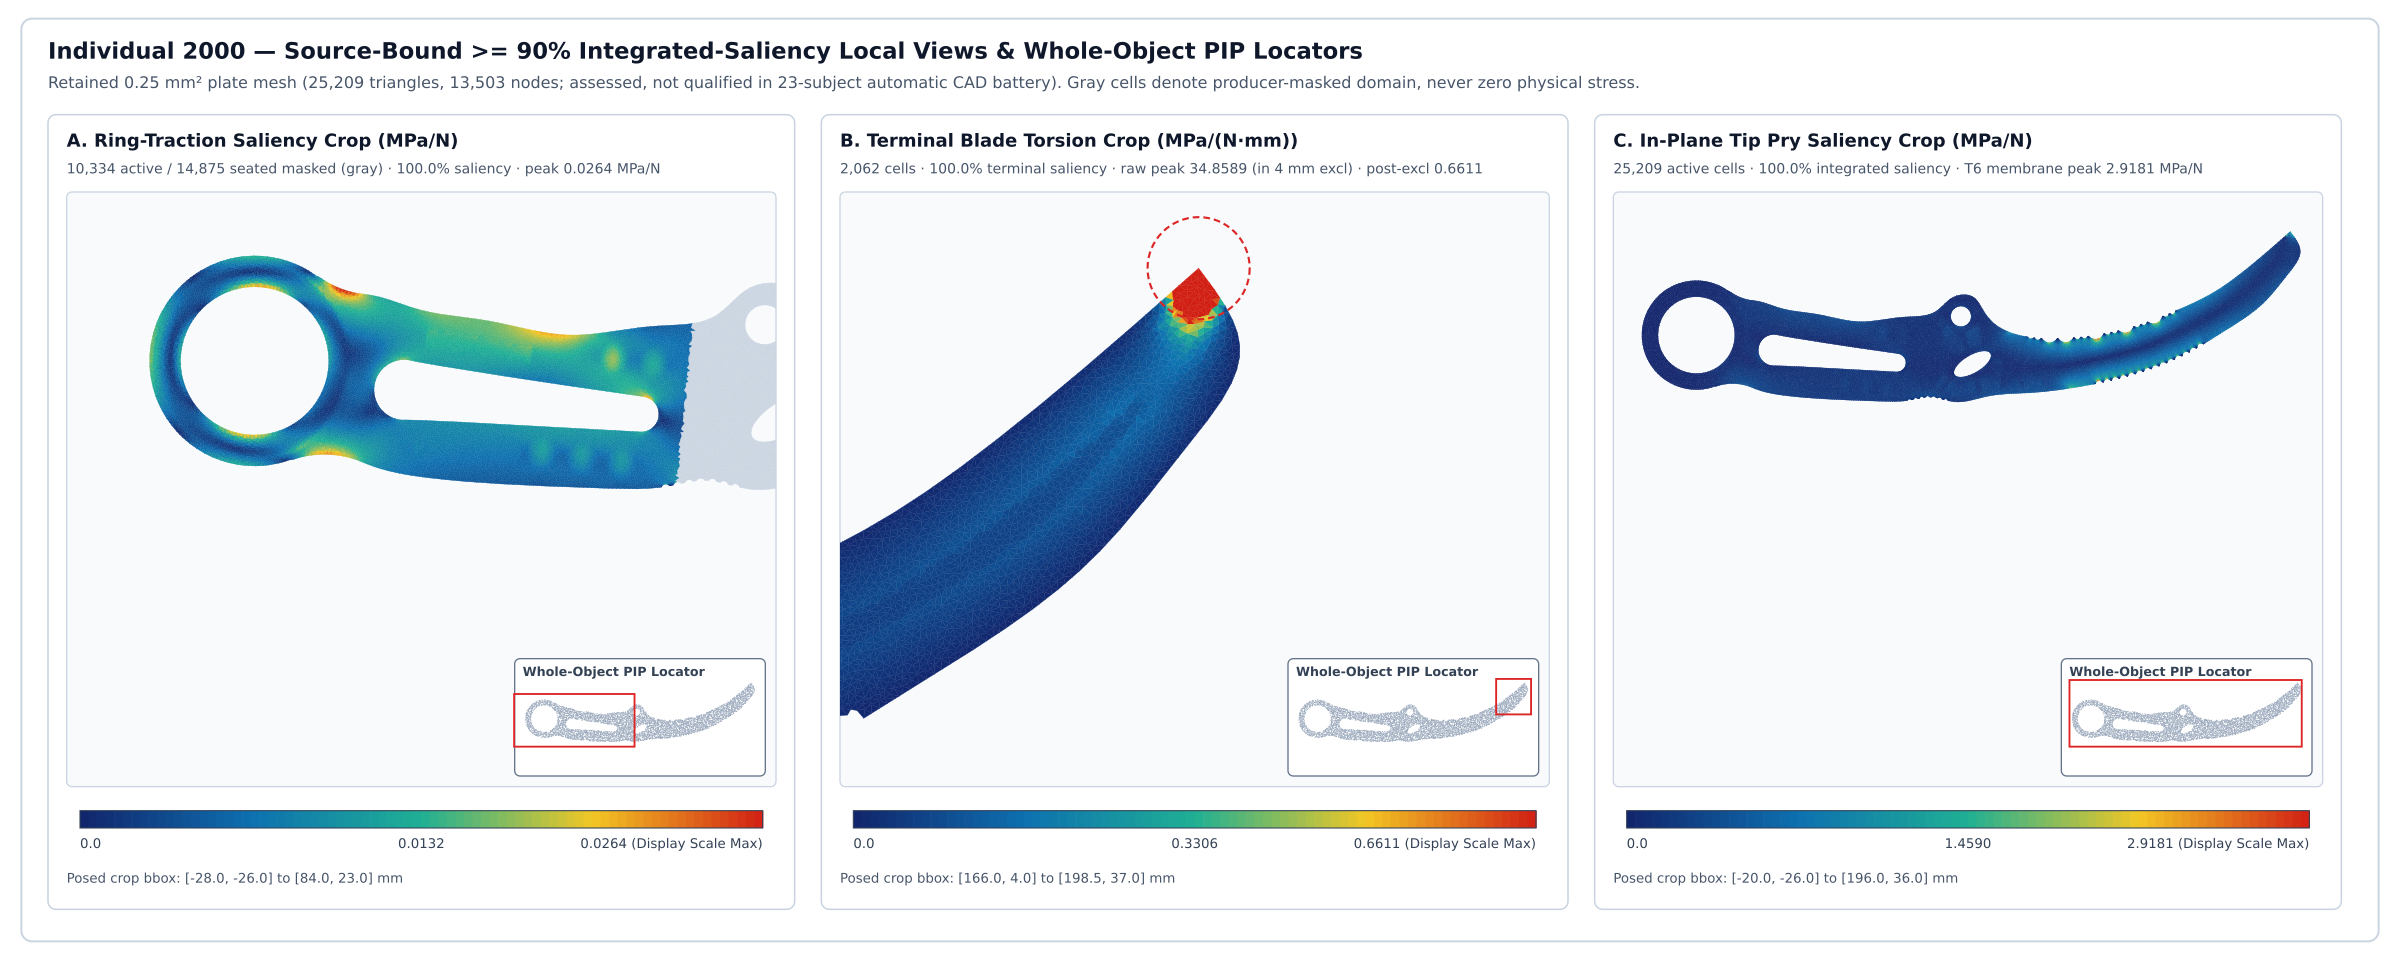
\includegraphics[width=\textwidth]{JR_EI_P4_T04_fem_saliency_crops_and_locators.png}
\caption{Source-bound $\ge 90\%$ integrated-saliency local views and whole-object picture-in-picture locators for Individual~2000 ($25{,}209$ triangles; assessed, not qualified). A: ring-traction unit response ($\mathrm{MPa/N}$) cropped to the $\ge 90\%$ area-weighted saliency bounding box over the $10{,}334$ unmasked ring/neck cells (retaining $100.0\%$ of integrated saliency, peak $0.0264\,\mathrm{MPa/N}$, and $14{,}875$ seated-ring masked cells rendered in neutral gray). B: terminal blade-tip chord-torsion unit response ($\mathrm{MPa/(N\,mm)}$) cropped to the $\ge 90\%$ saliency window (retaining $100.0\%$ of terminal saliency across $2{,}062$ cells, raw peak $34.8589\,\mathrm{MPa/(N\,mm)}$ inside the dashed $4\,\mathrm{mm}$ exclusion, and post-exclusion capacity peak $0.6611\,\mathrm{MPa/(N\,mm)}$). C: multi-case von Mises stress envelope ($\mathrm{MPa}$, retaining $99.8\%$ of integrated saliency across $23{,}659$ active cells, peak $1{,}388.6695\,\mathrm{MPa}$, and $75$ tip-excluded cells).}
\label{fig:saliency-crops}
\end{figure*}
